\documentclass[12pt, titlepage]{article}
\usepackage[utf8x]{inputenc}
\usepackage[english]{babel}
\usepackage[a4paper, top=3cm, bottom=2cm, left=2cm, right=2cm, marginparwidth=1.75cm, headheight=15pt]{geometry}
\usepackage{tabto}
\usepackage{fancyhdr}
\usepackage{titlesec}
\usepackage{float}
\usepackage{graphicx}
\usepackage{caption}
\usepackage[table]{xcolor}
\usepackage{parskip}
\definecolor{light-gray}{gray}{0.15}
\usepackage[colorlinks=true, allcolors=blue]{hyperref}

\newcommand{\code}[1]{\texttt{#1}}

\fancyhead[L]{\today}
\fancyhead[C]{SX-Dashboard Documentation}
\fancyhead[R]{MTechHub}
\pagestyle{fancy}

\setcounter{secnumdepth}{4}

\titleformat{\paragraph}
{\normalfont\normalsize\bfseries}{\theparagraph}{1em}{}
\titlespacing*{\paragraph}
{0pt}{3.25ex plus 1ex minus .2ex}{1.5ex plus .2ex}

\title{SX-Dashboard Documentation}
\author{MTechHub}
\date{\today}

\begin{document}

\setlength{\arrayrulewidth}{1.5pt}
\definecolor{table-grey}{gray}{0.90}

\maketitle
\newpage

\pagenumbering{roman}
\tableofcontents
\newpage
\pagenumbering{arabic}

\section{Project Overview}

\subsection{Application Walk-through}

\subsubsection{Adding packages}

Before the application can be run, it's dependencies must be installed. While in the project directory, run:\\
\code{npm install} or \code{yarn}\\
All the packages will be added to the folder /node\_modules. A list of dependencies can be found under ./package.json.

\subsubsection{Running the Application}

While in the project directory, run:\\
\code{npm start} or \code{yarn start}\\
to begin running the application at http://localhost:3000.\\

To build the application, run:\\
\code{npm build} or \code{yarn build}

\subsubsection{Using the Application}

After running the application, visit http://localhost:3000 in your browser. You should be redirected to http://localhost:3000/main/dashboard, and your screen should look similar to figure 1.

\begin{figure}[H]
\centering
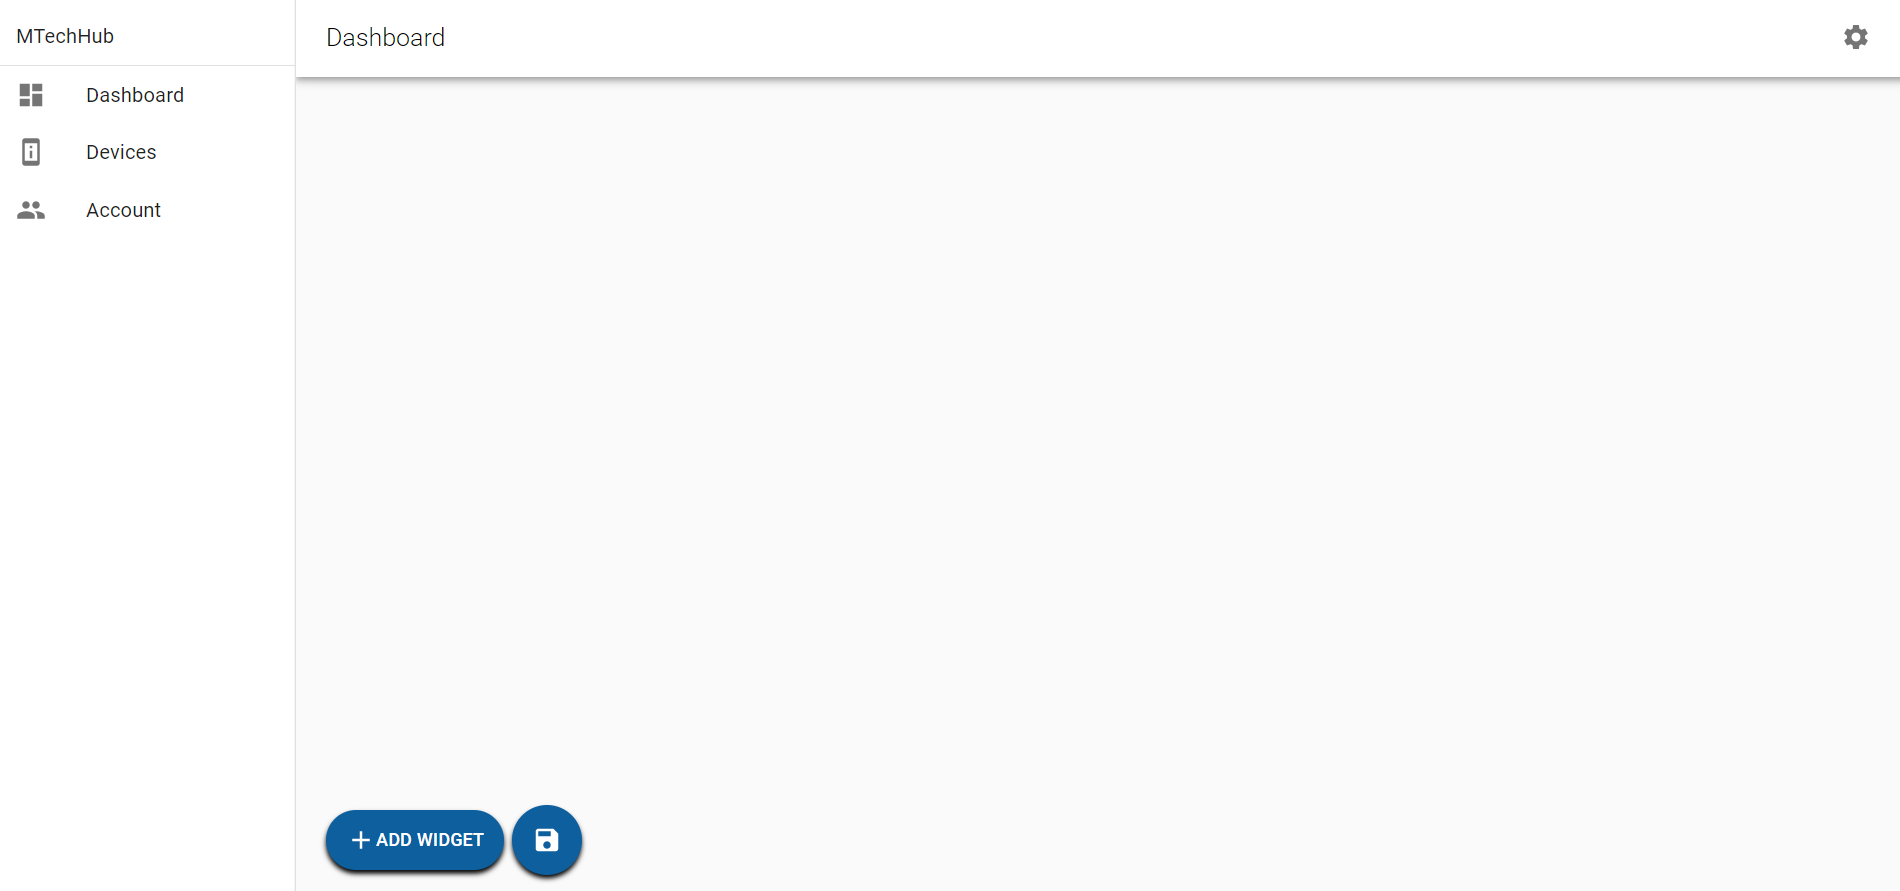
\includegraphics[width=0.9\linewidth]{./assets/Dash.PNG}
\caption{Starting screen}
\label{fig:dash}
\end{figure}

The Devices and Account tabs on the side are placeholders, and should be replaced with required tabs. Selecting Add Widget will bring up a menu with different chart types and a SQL/MQTT slider. The MQTT slider will setup a chart using the MQTT protocol to retrieve live data, whereas the SQL slider will setup a chart using a specified SQL database as the data source. Click the name of the chart you wish to create. A second menu will pop up asking for the relevant data, at the moment this is for show and the logic needs to be implemented. Fill in the required fields and select Create to create a chart.

Note that if creating a chart from SQL, at the moment it will give you a view of the last 10 records in that table, along with the column names so you can select the columns to create the chart from.

A chart should show up on the dashboard. This chart can be manipulated, click and drag to move it, drag the bottom-right corner to resize, and finally press the \textbf{X} in the top-right to delete the chart. Once you are finished with the layout of the dashboard, select the save icon to the right of Add Widget. This will save the layout to SQL, using the server API. At this point, closing the page and re-opening it should load up your last saved dashboard (assuming a successful SQL connection).

There is a cog icon located in the top right corner of the page. Currently this button does nothing, however it can be setup to contain a drop-down allowing customization (ex: theme selection by modifying the values used in theme.jsx).

\subsection{Code Walk-through}

All of the files mentioned here are found in /src/. Just about every react component will contain a render section: 
\begin{verbatim}
    render() {
        return (

        );
    }
\end{verbatim}
\noindent Anything here is what will be rendered whenever this component gets called by another file.  

\noindent The entry point for this project is ./index.js, which contains a router that essentially redirects to ./layout/main.jsx. Main.jsx is the main layout for the project, it just renders the Sidebar component found in ./components/sidebar/sidebar.jsx.

\textbf{The Sidebar Component}

\noindent Sidebar is the menu component found on the left side of the dashboard. When the screen size is md and lower, the menu is hidden and opens via a button placed at the top left of the appbar. The actual items on the sidebar menu are loaded in from ./components/items/. list\_items.jsx is rendered for the persistent sidebar, while mobile\_list\_items.jsx is rendered for the collapsible variant.

\noindent Each of the menu items has an associated path. This path is used in the Router found in the $<$main$>$ section within sidebar.jsx. It essentially loads the content in the main window of the application, and allows that content to change depending on which menu item has been selected.

\textbf{The Dashboard Component}

\noindent The dashboard, located under ./views/dashboard/dashboard.jsx is the default rendered view. componentDidMount() is called as soon as the component is mounted, in here is where we asynchronously make a call to SQL to retrieve the last-saved dashboard layout. In the case that there is no found layout from SQL, we attempt to use the last layout stored in localstorage. Else, the dashboard will be a blank slate.

\noindent There are functions for creating a chart, and creating the grid layout. It is fairly straightforward, the layout is rendered by mapping every item through the createElement function.  

\textbf{The Add Widget Popup}

\noindent There is a popup folder under components containing three files. They each create a separate dialog, for each stage of the widget creation process. Props \& References are used here, they simply allow you to access certain sections of the other popups. Conditional rendering is also used to allow for different popups depending on if MQTT or SQL is being used as the data source.

\textbf{Widgets}

\noindent Widgets are created using React-Google-Charts. Their documentation makes it quite easy to create any new charts you may require. Within the widgets folder, most are standard \& currently just using sample data. However, timeline.jsx shows how to customize tooltips, while also getting data from SQL. While gauge.jsx shows how to setup a websocket to retrieve MQTT data. 


\subsection{Project Structure}
\subsubsection{doc}

The doc folder contains this pdf and the .tex file used to generate it. Pdflatex is required to regenerate this document locally, however there are compilers online you can use as well if you ever need to make changes. Assets contains the images used in the document

\subsubsection{public}

The public contains your index.html file, a favicon \& a web app manifest. 

\subsubsection{src}

All the main code is found under src. The components folder contains all the different components to be used across the application. The server directory contains the golang code for most of the backend. Check the README for more info on what each go file does \& how to build.

\subsubsection{get\_view\_server\_files}

There was originally a separate server folder setup to test out getting the top 10 rows of a view, as well as saving \& retrieving layouts. 

\subsubsection{dotnet\_api\_files}

These are the c\# files created when converting from go to .net.  

\section{TODO List}

This project still has some additions required.

\begin{itemize}
\item When creating a chart, currently they just use sample data. They should be updated to use whatever data source is entered in the popups. One way to go about this would be to get the data source from the popup, and pass through an object containing this info as a prop when creating the widget (eg: \textless Timeline ds=\{data\_source\_var\}/\textgreater).
\item The popups where a user enters their SQL/MQTT data are currently just for show. Eventually you will need to send this to an API you've setup to access their database.
\item Finish up the MQTT portion of the .net file. Currently I have it working as an MQTT client, however it will need to connect to the broker we are using, and send data to the correct gauge widgets. \href{https://gist.github.com/prabirshrestha/2765381}{Refer to this gist as an example}.
\item The files in get\_view\_server\_files has not been transferred to .net yet. The go code for it should be clear and fairly easy to convert. These files handle the saving \& loading of the layout, as well as the preview when selecting from SQL.
\item Testing .net implementation of the main server files. They are converted and work when tested via Postman, however I did not have enough time to test it fully within the React App. Changing the fetch requests to use the go/.net APIs is very easy if you need to at any point.   
\item You may notice an error on the Timeline, saying "Invalid data table format". This is due to the Timeline not being able to reach the API where it gets it's data from.
\item Currently on load up there is a fetch called to api/get-view. I believe this is accidentally getting called early, as the popup where the view is displayed technically is mounted, just invisible. To fix this, you would have a boolean prop for whether it is visible yet, if true, then the fetch within componentDidMount should be allowed to run.  
\end{itemize}
\end{document}